\documentclass[tikz,border=10pt]{standalone}
\usetikzlibrary{shapes.geometric, positioning, arrows.meta, scopes, patterns, shadows, calc}

\usepackage{xstring}

\def\code#1{\color{olive}{\texttt{#1}}\color{black}~}
% \def\refer#1{Fig. \ref{#1}}
% \newcommand{\urlpath}[1]{%
% \begin{FVerbatim}[fontsize=\scriptsize]
% #1
% \end{FVerbatim}%
% }

\def\comment#1{\color{olive}{\textit{\% #1}} \color{black}}

\newcommand\ezeq[1]{$#1$}

\newcommand\ezcolumn[3]{
\begin{column}{#1\textwidth}
    \vspace{#2cm}
    #3
\end{column}
}

% \newenvironment{myenumerate}{%
%   \begin{enumerate}
%     \renewcommand{\theenumii}{\arabic{enumi}.\arabic{enumii}}
%   }
%   {%
%   \end{enumerate}
% }


\newcommand{\customenumerate}{%
  \renewcommand{\theenumii}{\arabic{enumi}.\arabic{enumii}}
  \renewcommand{\theenumiii}{\arabic{enumi}.\arabic{enumii}.\arabic{enumiii}}
}


\begin{document}
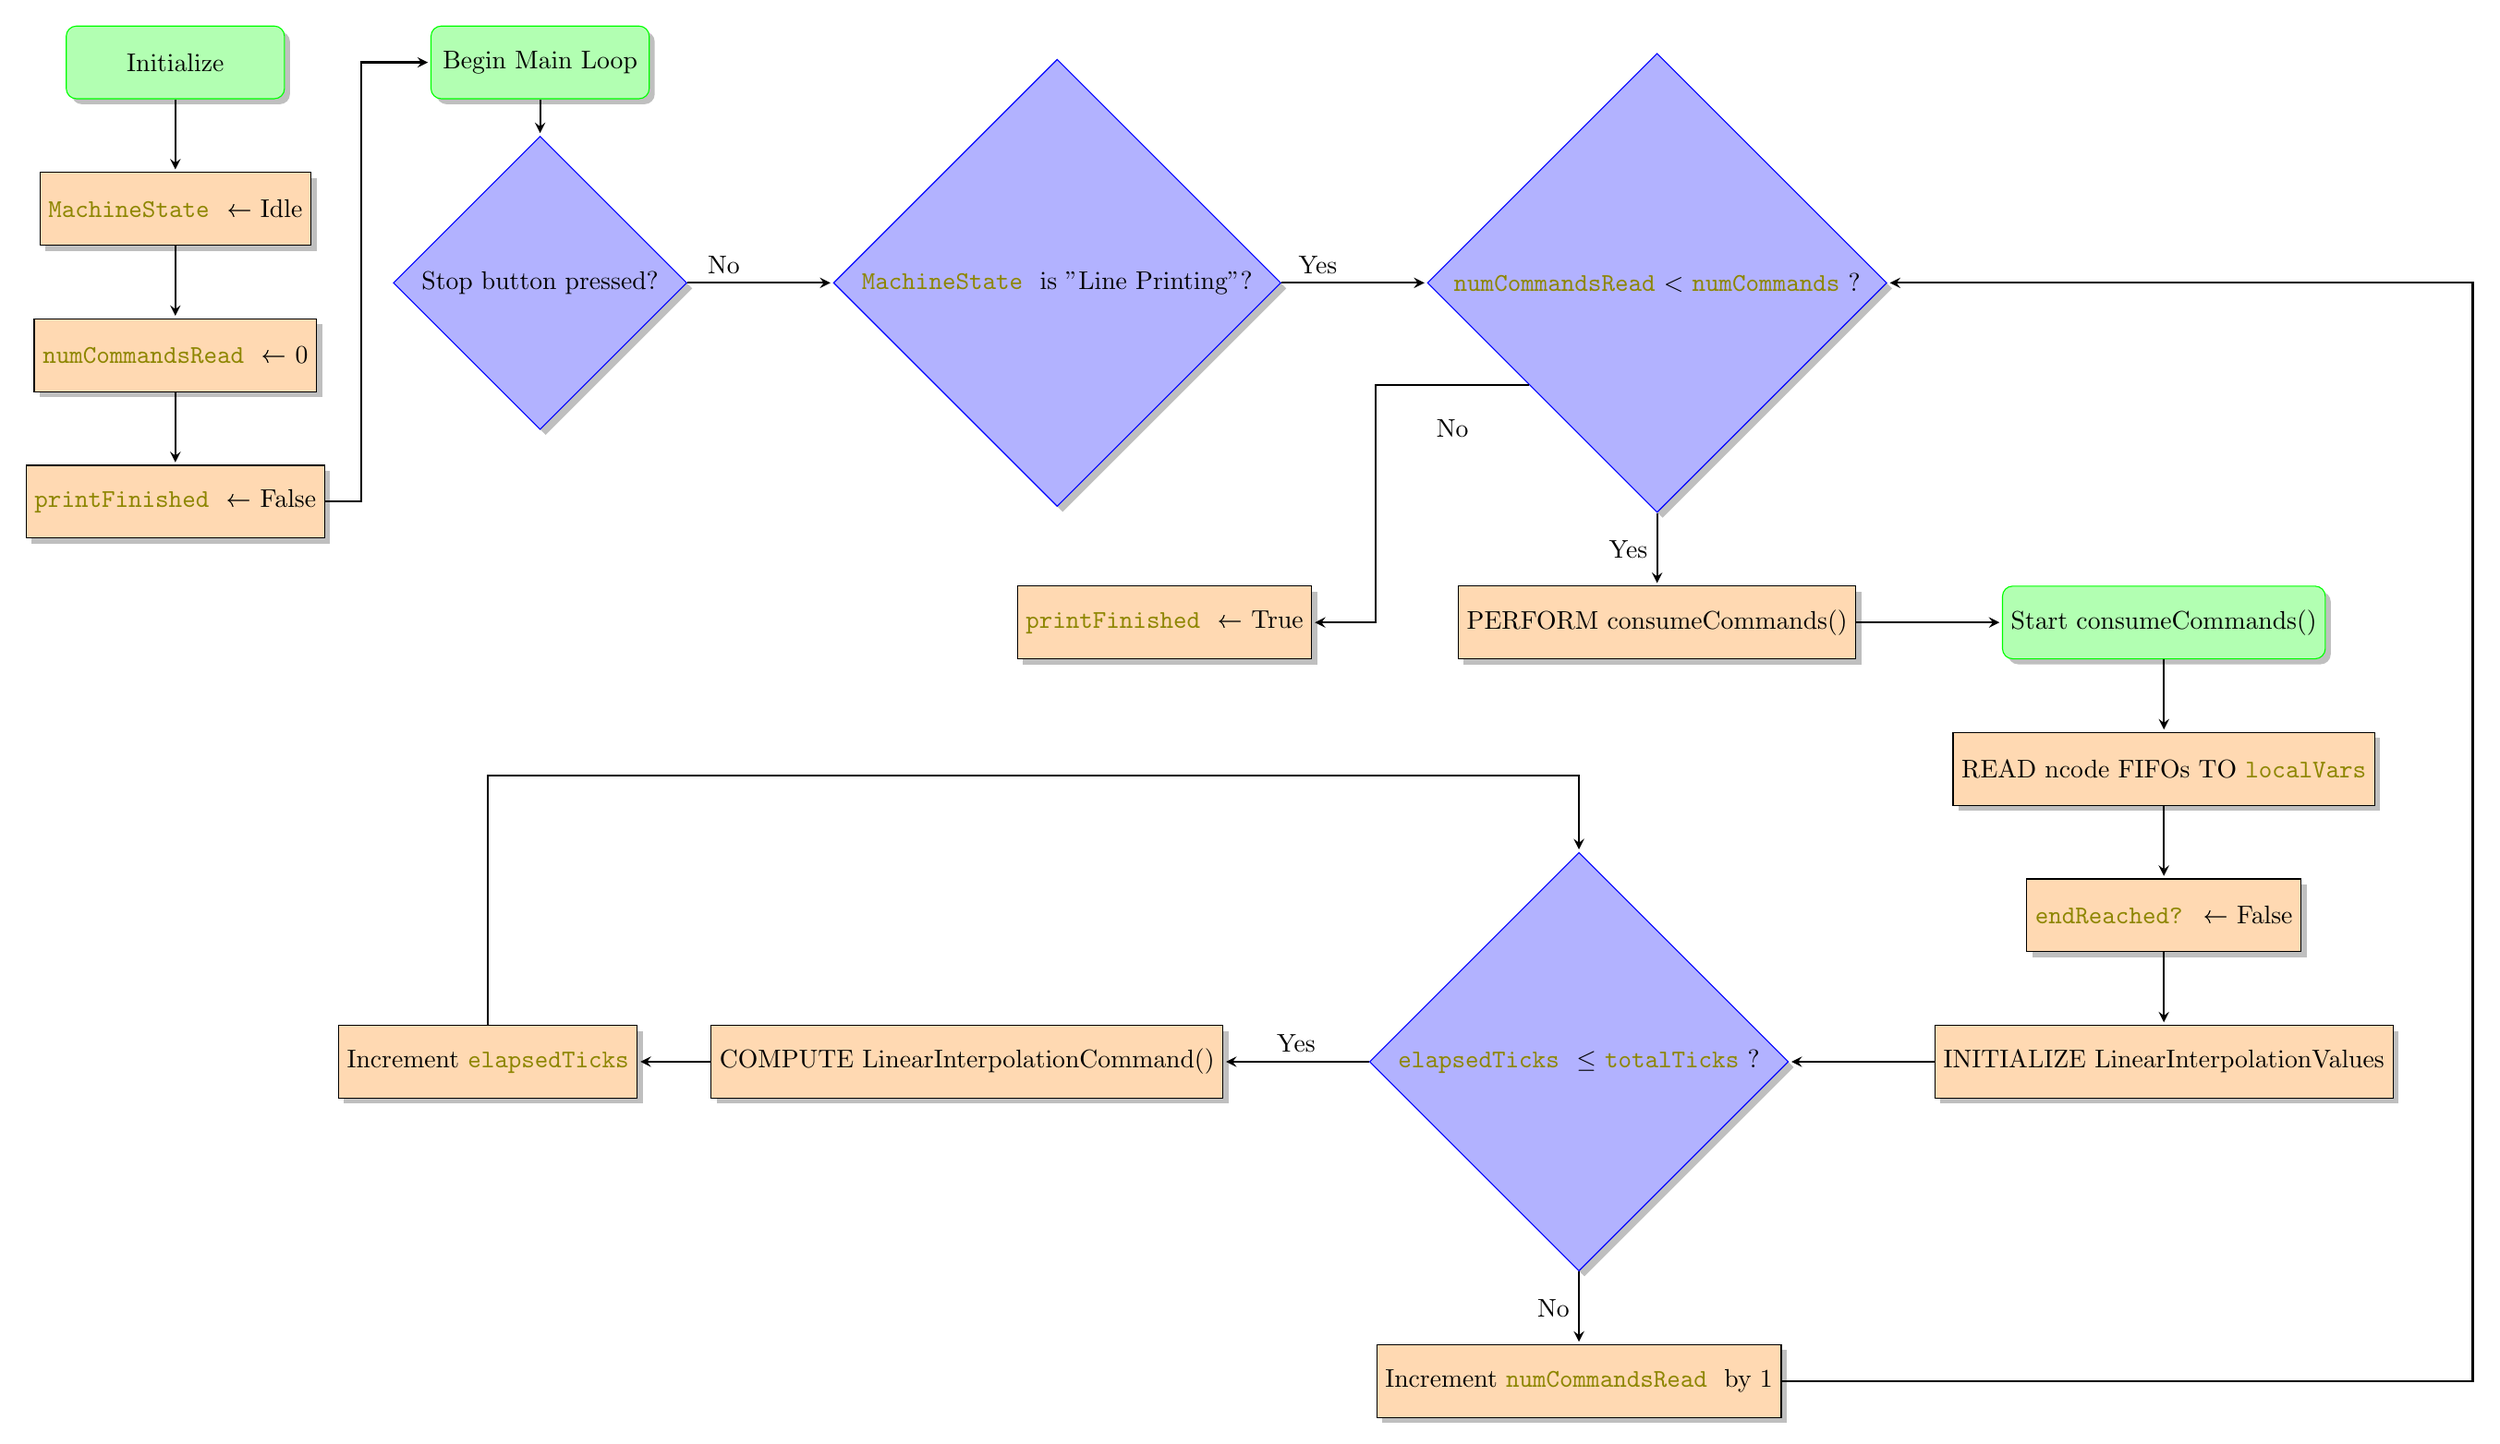
\begin{tikzpicture}[
    startstop/.style={rectangle, rounded corners, minimum width=3cm, minimum height=1cm, text centered, draw=green, fill=green!30, drop shadow},
    process/.style={rectangle, minimum width=3cm, minimum height=1cm, text centered, draw=black, fill=orange!30, drop shadow},
    io/.style={trapezium, trapezium left angle=70, trapezium right angle=110, minimum width=3cm, minimum height=1cm, text centered, draw=blue, fill=blue!30, drop shadow},
    decision/.style={diamond, minimum width=3cm, minimum height=1.5cm, text centered, draw=blue, fill=blue!30, drop shadow},
    arrow/.style={thick,->,>=stealth, shorten >=1pt},
]

% Initialize
\node[startstop] (init) {Initialize};
\node[process, below=1cm of init] (setMachine) {\code{MachineState} ← Idle};
\node[process, below=1cm of setMachine] (setNumCmd) {\code{numCommandsRead} ← 0};
\node[process, below=1cm of setNumCmd] (setPrint) {\code{printFinished} ← False};

% Begin Main Loop
\node[startstop, right=2cm of init] (mainLoop) {Begin Main Loop};
\node[decision, below=0.5cm of mainLoop] (chkStopButton) {Stop button pressed?};
\node[decision, right=2cm of chkStopButton] (chkState) {\code{MachineState} is "Line Printing"?};
\node[decision, right=2cm of chkState] (chkCmd) {\code{numCommandsRead}\ezeq{<} \code{numCommands}?};
\node[process, below=1cm of chkCmd] (consumeCommands) {PERFORM consumeCommands()};
\node[process, left=2cm of consumeCommands] (setPrintFin) {\code{printFinished} ← True};

% Procedure consumeCommands
\node[startstop, right=2cm of consumeCommands] (startConsumeCommands) {Start consumeCommands()};
\node[process, below=1cm of startConsumeCommands] (readNcode) {READ ncode FIFOs TO \code{localVars}};
\node[process, below=1cm of readNcode] (assumeEnd) {\code{endReached?} ← False};
\node[process, below=1cm of assumeEnd] (initLin) {INITIALIZE LinearInterpolationValues};
\node[decision, left=2cm of initLin] (checkTicks) {\code{elapsedTicks} \ezeq{\leq} \code{totalTicks}?};
\node[process, left=2cm of checkTicks] (computeInterpolation) {COMPUTE LinearInterpolationCommand()};
\node[process, left=1cm of computeInterpolation] (incrementTicks) {Increment \code{elapsedTicks}};
\node[process, below=1cm of checkTicks] (incrementCmd) {Increment \code{numCommandsRead} by 1};

% Arrows for Initialize
\draw[arrow] (init) -- (setMachine);
\draw[arrow] (setMachine) -- (setNumCmd);
\draw[arrow] (setNumCmd) -- (setPrint);
\draw[arrow] let \p1 = (setPrint.east), \p2 = (mainLoop.west) in 
    (\p1) -- ++(0.5,0) |- (\x2,\y2);
% (setPrint) -- ++(2,0) |- (mainLoop);

% Arrows for Main Loop
\draw[arrow] (mainLoop) -- (chkStopButton);
\draw[arrow] let \p1 = (chkStopButton.east), \p2 = (chkState.west) in 
    (\p1) -- node[anchor=south, pos=1] {No} ++(0.5,0) |- (\x2,\y2);
(chkStopButton) -- node[anchor=east] {No} ++(0,-1.5cm) -| (chkState);
% \draw[arrow] (chkStopButton.east) -- node[anchor=north] {Yes} ++(3,0) |- (setPrintFin.west);
\draw[arrow] (chkState) -- node[anchor=south, pos=0.25] {Yes} (chkCmd);
\draw[arrow] (chkCmd) -- node[anchor=east] {Yes} (consumeCommands);
% \draw[arrow] (chkCmd) -- node[anchor=north,yshift=-10pt] {No} (setPrintFin);
\draw[arrow] 
  let \p1 = (chkCmd.west), \n1 = {\x1 + 40pt}, \n2 = {\y1 - 40pt}, \p2 = (setPrintFin.east) in 
  (\n1,\n2) -- node[anchor=north,yshift=-10pt] {No} (\n1 - 60pt,\n2) -- (\n1 - 60pt, \y2) -- (\p2);
\draw[arrow] (consumeCommands) -- (startConsumeCommands);

% Arrows for Procedure consumeCommands
\draw[arrow] (startConsumeCommands) -- (readNcode);
\draw[arrow] (readNcode) -- (assumeEnd);
\draw[arrow] (assumeEnd) -- (initLin);
\draw[arrow] (initLin) -- (checkTicks);
\draw[arrow] (checkTicks) -- node[anchor=south] {Yes} (computeInterpolation);
\draw[arrow] (checkTicks) -- node[anchor=east] {No} (incrementCmd);
\draw[arrow] (computeInterpolation) -- (incrementTicks);
\draw[arrow] let \p1 = (incrementTicks.north), \p2 = (checkTicks.north) in 
    (\p1) -- (\x1,\y2 + 30pt) -- (\x2,\y2 + 30pt) -- (\p2);
\draw[arrow] let \p1 = (incrementCmd.east), \p2 = (chkCmd.east) in 
    (\p1) -- ++(9.5,0) |- (\x2,\y2);

\end{tikzpicture}
\end{document}
